\documentclass{standalone}
\usepackage{pgfplots}
\begin{document}
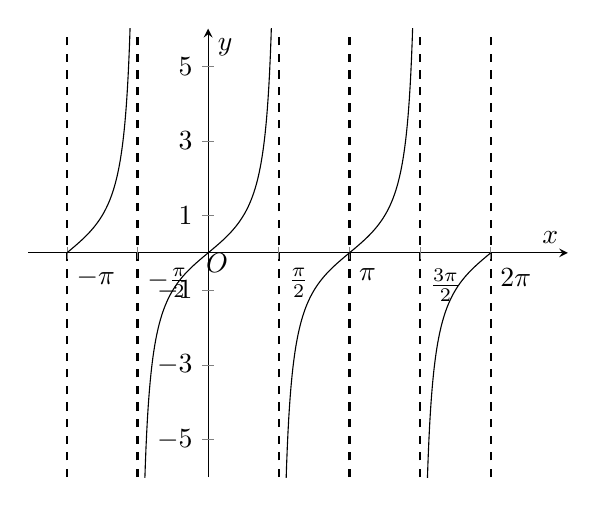
\begin{tikzpicture}
\begin{axis}
[
ymin=-6,ymax=6,
xmin=-4,xmax=8,
%clip=false,
xtick=\empty,
ytick=\empty,
extra x ticks={-3.1416, -1.5708, 1.5708, 3.1416, 4.71239, 6.2832},
extra x tick labels={$-\pi$, $-\frac{\pi}{2}$, $\frac{\pi}{2}$, $\pi$, $\frac{3\pi}{2}$, $2\pi$},
extra y ticks={-5, -3, -1, 1, 3, 5},
extra y tick labels={$-5$, $-3$, $-1$, $1$, $3$, $5$},
every extra x tick/.style={
    xticklabel style={anchor=north west},
    grid=major,
    major grid style={thick,dashed,black}
},
axis lines = center,
xlabel=$x$,ylabel=$y$,
domain=-.5*pi:.5*pi,
samples=200,
]
\addplot [black] {tan(deg(x))};
\addplot [domain=pi/2:3*pi/2] {tan(deg(x))};
\addplot [domain=3*pi/2:2*pi] {tan(deg(x))};
\addplot [domain=-pi:-pi/2] {tan(deg(x))};
\node at (axis cs:0.2, -0.28) {$O$} ;
\end{axis}
\end{tikzpicture}
\end{document}
